\documentclass[11pt]{article}
\usepackage[utf8]{inputenc}
\usepackage[margin=1in]{geometry}
\usepackage{tikz}
\usetikzlibrary{shapes.geometric, arrows.meta, positioning}
\usepackage{listings}
\usepackage{xcolor}
\usepackage{booktabs}
\usepackage{longtable}
\usepackage{amsmath}
\usepackage{amssymb}
\usepackage{microtype}
\usepackage{enumitem}
\usepackage{hyperref}
\sloppy

\lstset{
    language=SQL,
    basicstyle=\ttfamily\scriptsize,
    keywordstyle=\color{blue}\bfseries,
    stringstyle=\color{red},
    commentstyle=\color{gray},
    breaklines=true,
    frame=single,
    showstringspaces=false
}

\lstdefinelanguage{Python}{
    keywords={def, return, if, else, elif, with, as, import, from, for, in, not, and, or, True, False, None, await, async, try, except, class},
    keywordstyle=\color{blue}\bfseries,
    ndkeywords={self, request, connection, transaction, cursor, execute, fetchone, fetchall},
    ndkeywordstyle=\color{purple},
    stringstyle=\color{red},
    commentstyle=\color{gray}\itshape,
    morecomment=[l]{\#},
    morestring=[b]',
    morestring=[b]",
}

\lstdefinelanguage{JavaScript}{
    keywords={function, return, if, else, const, let, var, async, await, export, import, from, try, catch, throw, new, this, class, extends, default},
    keywordstyle=\color{blue}\bfseries,
    ndkeywords={useState, useEffect, useRef, fetch, JSON, console, document, window},
    ndkeywordstyle=\color{purple},
    stringstyle=\color{red},
    commentstyle=\color{gray}\itshape,
    morecomment=[l]{//},
    morestring=[b]',
    morestring=[b]",
    morestring=[b]`,
}

\title{Database Project Report 2 \\ \large CS6083 Spring 2026 \\ \large snickr: A Web-Based Collaboration System}
\author{
    \begin{tabular}[t]{c}
        Christine Wagner \\
        \texttt{caw561@nyu.edu}
    \end{tabular}
    \hspace{2em}
    \begin{tabular}[t]{c}
        Hongyi Zeng \\
        \texttt{hz3866@nyu.edu}
    \end{tabular}
}
\date{\today}

\begin{document}

\maketitle

\tableofcontents
\newpage

%% ================================================================
%%  PART 1 --- DATABASE DESIGN (revised from Project 1)
%% ================================================================

\section{Introduction}

This report documents the design and implementation of \textit{snickr}, a web-based collaboration system inspired by Slack. The system allows users to create workspaces, organize communication through public, private, and direct channels, and exchange messages within those channels.

The database is built on PostgreSQL~15 and consists of six relations: \texttt{users}, \texttt{workspaces}, \texttt{workspace\_members}, \texttt{channels}, \texttt{channel\_members}, and \texttt{messages}. Access control is enforced at the application level --- a single DBMS account is used, and the application restricts content visibility based on workspace and channel membership.

This report covers both Project~1 (schema design and queries) and Project~2 (web interface implementation). Section~\ref{sec:schema} presents the database schema design with ER diagrams. Section~\ref{sec:creation} provides the schema creation SQL. Section~\ref{sec:queries} documents the seven required queries. Section~\ref{sec:testdata} discusses the test data. Sections~\ref{sec:arch}--\ref{sec:session} cover the Project~2 web application: architecture, implementation details, security measures, concurrency handling, user guide, and sample session logs. Section~\ref{sec:revisions} discusses design decisions and revisions made for Project~2. Section~\ref{sec:extra} describes additional features implemented for extra credit.

The full source code is available at: \url{https://github.com/MacroMozilla/DBProject}


\section{Database Schema Design}
\label{sec:schema}

\subsection{ER Diagram}

\begin{center}
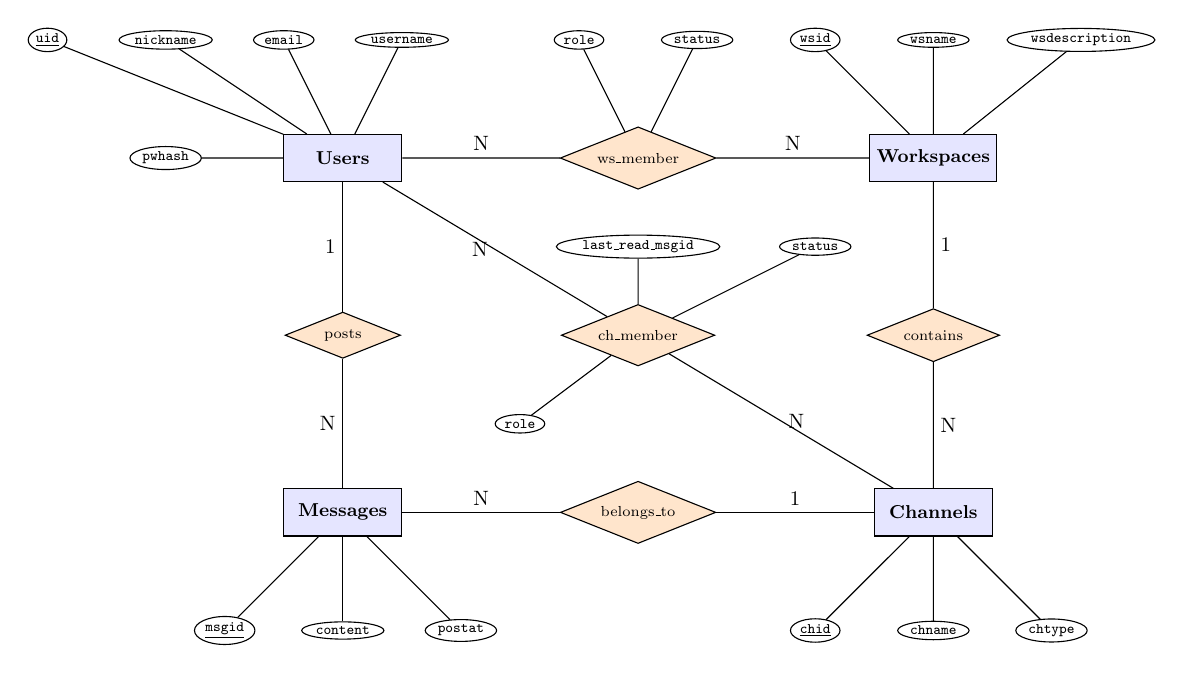
\begin{tikzpicture}[
    entity/.style={rectangle, draw, fill=blue!10, minimum width=2cm, minimum height=0.8cm, font=\small\bfseries},
    relationship/.style={diamond, draw, fill=orange!20, aspect=2.5, font=\scriptsize},
    attr/.style={ellipse, draw, fill=white, inner sep=1pt, font=\scriptsize\ttfamily},
    >=Stealth,
    scale=0.75, transform shape
]

% Row 1: Entities
\node[entity] (user) at (0, 6) {Users};
\node[entity] (workspace) at (10, 6) {Workspaces};
\node[entity] (channel) at (10, 0) {Channels};
\node[entity] (message) at (0, 0) {Messages};

% Row 2: Relationships (links in the middle)
\node[relationship] (wm) at (5, 6) {ws\_member};
\node[relationship] (cm) at (5, 3) {ch\_member};
\node[relationship] (posts) at (0, 3) {posts};
\node[relationship] (contains) at (10, 3) {contains};
\node[relationship] (belongsto) at (5, 0) {belongs\_to};

% User attributes (above and left)
\node[attr] (uuid) at (-5, 8) {\underline{uid}};
\node[attr] (uemail) at (-1, 8) {email};
\node[attr] (uname) at (1, 8) {username};
\node[attr] (unick) at (-3, 8) {nickname};
\node[attr] (upw) at (-3, 6) {pwhash};

% Workspace attributes (above and right)
\node[attr] (wsid) at (8, 8) {\underline{wsid}};
\node[attr] (wsname) at (10, 8) {wsname};
\node[attr] (wsdesc) at (12.5, 8) {wsdescription};

% Channel attributes (below and right)
\node[attr] (chid) at (8, -2) {\underline{chid}};
\node[attr] (chname) at (10, -2) {chname};
\node[attr] (chtype) at (12, -2) {chtype};

% Message attributes (below and left)
\node[attr] (msgid) at (-2, -2) {\underline{msgid}};
\node[attr] (content) at (0, -2) {content};
\node[attr] (postat) at (2, -2) {postat};

% ws_member attributes (above the diamond)
\node[attr] (wmrole) at (4, 8) {role};
\node[attr] (wmstatus) at (6, 8) {status};

% ch_member attributes (sides of the diamond)
\node[attr] (cmrole) at (3, 1.5) {role};
\node[attr] (cmstatus) at (8, 4.5) {status};
\node[attr] (cmread) at (5, 4.5) {last\_read\_msgid};

% Edges: User attributes
\draw (user) -- (uuid);
\draw (user) -- (uemail);
\draw (user) -- (uname);
\draw (user) -- (unick);
\draw (user) -- (upw);

% Edges: Workspace attributes
\draw (workspace) -- (wsid);
\draw (workspace) -- (wsname);
\draw (workspace) -- (wsdesc);

% Edges: Channel attributes
\draw (channel) -- (chid);
\draw (channel) -- (chname);
\draw (channel) -- (chtype);

% Edges: Message attributes
\draw (message) -- (msgid);
\draw (message) -- (content);
\draw (message) -- (postat);

% Edges: Relationship attributes
\draw (wm) -- (wmrole);
\draw (wm) -- (wmstatus);
\draw (cm) -- (cmrole);
\draw (cm) -- (cmstatus);
\draw (cm) -- (cmread);

% Edges: Entity-Relationship connections
\draw (user) -- node[above] {N} (wm);
\draw (workspace) -- node[above] {N} (wm);
\draw (user) -- node[left] {N} (cm);
\draw (channel) -- node[right] {N} (cm);
\draw (user) -- node[left] {1} (posts);
\draw (posts) -- node[left] {N} (message);
\draw (workspace) -- node[right] {1} (contains);
\draw (contains) -- node[right] {N} (channel);
\draw (message) -- node[above] {N} (belongsto);
\draw (belongsto) -- node[above] {1} (channel);

\end{tikzpicture}
\end{center}

\subsection{Relational Schema}

The ER diagram translates into the following six relations:

\begin{enumerate}
\item \textbf{users}(\underline{uid}, email, username, nickname, pwhash, createdat, updatedat)
\begin{itemize}
\item email is \texttt{UNIQUE NOT NULL}
\end{itemize}

\item \textbf{workspaces}(\underline{wsid}, wsname, wsdescription, createdat, updatedat)

\item \textbf{workspace\_members}(\underline{wsid}, \underline{uid}, role, status, createdat, updatedat)
    \begin{itemize}
        \item wsid $\rightarrow$ workspaces(wsid)
        \item uid $\rightarrow$ users(uid)
        \item role $\in$ \{creator, admin, member\}
        \item status $\in$ \{pending, accepted, rejected\}
    \end{itemize}

\item \textbf{channels}(\underline{chid}, wsid, chname, chtype, createdat, updatedat)
    \begin{itemize}
        \item wsid $\rightarrow$ workspaces(wsid)
        \item chtype $\in$ \{public, private, direct\}
    \end{itemize}

\item \textbf{channel\_members}(\underline{chid}, \underline{uid}, role, status, last\_read\_msgid, createdat, updatedat)
    \begin{itemize}
        \item chid $\rightarrow$ channels(chid)
        \item uid $\rightarrow$ users(uid)
        \item role $\in$ \{creator, member\}
        \item status $\in$ \{pending, accepted, rejected\}
    \end{itemize}

\item \textbf{messages}(\underline{msgid}, chid, uid, content, postat)
    \begin{itemize}
        \item chid $\rightarrow$ channels(chid)
        \item uid $\rightarrow$ users(uid)
    \end{itemize}

\end{enumerate}

\subsection{Normalization Analysis}

All six relations are in \textbf{BCNF (Boyce--Codd Normal Form)}:

\begin{itemize}
    \item \textbf{users}: The only candidate key is \texttt{uid} (surrogate). \texttt{email} is also a candidate key. Every non-trivial functional dependency has a superkey as its determinant. $\Rightarrow$ BCNF.
    \item \textbf{workspaces}: Single candidate key \texttt{wsid}. All attributes depend on \texttt{wsid}. $\Rightarrow$ BCNF.
    \item \textbf{workspace\_members}: Composite key \texttt{(wsid, uid)}. The attributes \texttt{role}, \texttt{status}, \texttt{createdat}, \texttt{updatedat} are fully functionally dependent on the composite key. No partial or transitive dependencies. $\Rightarrow$ BCNF.
    \item \textbf{channels}: Single candidate key \texttt{chid}. \texttt{wsid} is a foreign key, not a determinant of other attributes. $\Rightarrow$ BCNF.
    \item \textbf{channel\_members}: Composite key \texttt{(chid, uid)}. Same reasoning as \texttt{workspace\_members}. $\Rightarrow$ BCNF.
    \item \textbf{messages}: Single candidate key \texttt{msgid}. All attributes depend on \texttt{msgid}. $\Rightarrow$ BCNF.
\end{itemize}


\subsection{Design Assumptions}

\begin{itemize}
\item \textbf{A surrogate \texttt{uid} is used as the primary key for users}, rather than \texttt{email}. This allows users to change their email address without cascading updates across all foreign keys. The \texttt{email} column is constrained as \texttt{UNIQUE NOT NULL}.
\item \textbf{Creator is stored in membership tables, not in workspace/channel tables.} The creator is the first member inserted with role = \texttt{'creator'}. As specified in the requirements, the creator is treated as the initial administrator; query~(3) therefore includes both \texttt{'creator'} and \texttt{'admin'} roles when listing administrators. Storing the creator as a role avoids redundancy and simplifies queries.
\item \textbf{Invitations are tracked via the \texttt{status} field}, not as a separate entity. When a user is invited to a workspace or channel, a membership record is inserted with \texttt{status = 'pending'}. Upon acceptance, it is updated to \texttt{'accepted'}, and users may also explicitly decline an invitation by setting \texttt{'rejected'}. This design supports richer user interaction without introducing a separate invitations table.
\item \textbf{Public channels are visible to all workspace members but still require explicit membership.} Users are not automatically added upon channel creation; instead, they must choose to join. When a user joins a public channel, a record is inserted into \texttt{channel\_members} with \texttt{status = 'accepted'}, granting access to the channel's messages.
\item \textbf{Passwords are stored as SHA-256 hashes.} The \texttt{pwhash} field stores a hashed password rather than plaintext for security.
\item \textbf{Timestamps are recorded for all actions.} All tables include \texttt{createdat} and \texttt{updatedat} fields (messages use \texttt{postat} instead). While \texttt{updatedat} is not exercised by the required queries, it is included to support features such as profile edits, role changes, and invitation acceptance tracking.
\item \textbf{Member removal} is supported by deleting the corresponding row from \texttt{workspace\_members} or \texttt{channel\_members}. No soft-delete flag is needed since the membership record itself represents the relationship.
\item \textbf{Direct channels are limited to two members}, enforced at the application level rather than via a database constraint, since a \texttt{CHECK} on member count would require a trigger.
\item \textbf{Message read state is tracked at the channel level.} Each \texttt{channel\_members} record includes a \texttt{last\_read\_msgid} attribute, which stores the most recent message viewed by the user in that channel.
\item \textbf{Access control is enforced at the application level}, not through database permissions or views, as specified in the project requirements.
\end{itemize}

\subsection{Application-Level Enforcement}

The following constraints are enforced by the web application rather than the database, either because SQL \texttt{CHECK} constraints cannot express them without triggers, or because they involve session state:

\begin{itemize}
\item \textbf{Direct channel membership limit.} The application ensures that exactly two users are associated with a direct channel at creation time.
\item \textbf{Workspace invitation authority.} Only users with \texttt{role IN ('creator', 'admin')} in \texttt{workspace\_members} are permitted to insert new membership records for other users.
\item \textbf{Private channel invitation authority.} Only the channel creator (\texttt{role = 'creator'} in \texttt{channel\_members}) may invite additional users to a private channel.
\item \textbf{Session identification.} Each HTTP request includes a session cookie identifying the logged-in user \texttt{uid}. The application resolves this identity before executing any query.
\item \textbf{Public channel join eligibility.} Before inserting a \texttt{channel\_members} row for a public channel, the application verifies that the user has \texttt{status = 'accepted'} in the corresponding \texttt{workspace\_members} relation.
\end{itemize}


\subsection{Space Efficiency}

\begin{itemize}
    \item \textbf{No redundant creator columns.} Instead of storing a separate \texttt{creator\_uid} in the \texttt{workspaces} and \texttt{channels} tables, we encode the creator as a membership record with \texttt{role = 'creator'}.
    \item \textbf{Composite primary keys} on \texttt{workspace\_members} and \texttt{channel\_members} eliminate the need for surrogate ID columns in junction tables.
    \item \textbf{\texttt{VARCHAR} with appropriate limits} is used instead of fixed-length \texttt{CHAR} fields, so shorter values do not waste space.
    \item \textbf{\texttt{SERIAL} auto-increment} is used for \texttt{uid}, \texttt{wsid}, \texttt{chid}, and \texttt{msgid} (4-byte integers), which is more compact than UUIDs.
    \item \textbf{No separate invitations table.} The \texttt{status} field on membership tables tracks invitation state in-place, avoiding an extra table and the joins it would require.
\end{itemize}



\newpage
\section{Schema Creation}
\label{sec:creation}

The following SQL creates the schema in PostgreSQL with all key, foreign key, and check constraints:

\begin{lstlisting}
CREATE TABLE users (
    uid         SERIAL       PRIMARY KEY,
    email       VARCHAR(255) NOT NULL UNIQUE,
    username    VARCHAR(50)  NOT NULL,
    nickname    VARCHAR(50),
    pwhash      VARCHAR(255) NOT NULL,
    createdat   TIMESTAMP    NOT NULL DEFAULT CURRENT_TIMESTAMP,
    updatedat   TIMESTAMP    NOT NULL DEFAULT CURRENT_TIMESTAMP
);

CREATE TABLE workspaces (
    wsid        SERIAL       PRIMARY KEY,
    wsname      VARCHAR(100) NOT NULL,
    wsdescription TEXT,
    createdat   TIMESTAMP    NOT NULL DEFAULT CURRENT_TIMESTAMP,
    updatedat   TIMESTAMP    NOT NULL DEFAULT CURRENT_TIMESTAMP
);

CREATE TABLE workspace_members (
    wsid        INT          NOT NULL REFERENCES workspaces(wsid) ON DELETE CASCADE,
    uid         INT          NOT NULL REFERENCES users(uid) ON DELETE CASCADE,
    role        VARCHAR(10)  NOT NULL CHECK (role IN ('creator', 'admin', 'member')),
    status      VARCHAR(10)  NOT NULL CHECK (status IN ('pending', 'accepted', 'rejected'))
                             DEFAULT 'pending',
    createdat   TIMESTAMP    NOT NULL DEFAULT CURRENT_TIMESTAMP,
    updatedat   TIMESTAMP    NOT NULL DEFAULT CURRENT_TIMESTAMP,
    PRIMARY KEY (wsid, uid)
);

CREATE TABLE channels (
    chid        SERIAL       PRIMARY KEY,
    wsid        INT          NOT NULL REFERENCES workspaces(wsid) ON DELETE CASCADE,
    chname      VARCHAR(100),
    chtype      VARCHAR(10)  NOT NULL CHECK (chtype IN ('public', 'private', 'direct')),
    createdat   TIMESTAMP    NOT NULL DEFAULT CURRENT_TIMESTAMP,
    updatedat   TIMESTAMP    NOT NULL DEFAULT CURRENT_TIMESTAMP
);

CREATE TABLE channel_members (
    chid        INT          NOT NULL REFERENCES channels(chid) ON DELETE CASCADE,
    uid         INT          NOT NULL REFERENCES users(uid) ON DELETE CASCADE,
    role        VARCHAR(10)  NOT NULL CHECK (role IN ('creator', 'member')),
    status      VARCHAR(10)  NOT NULL CHECK (status IN ('pending', 'accepted', 'rejected'))
                             DEFAULT 'pending',
    last_read_msgid INT,
    createdat   TIMESTAMP    NOT NULL DEFAULT CURRENT_TIMESTAMP,
    updatedat   TIMESTAMP    NOT NULL DEFAULT CURRENT_TIMESTAMP,
    PRIMARY KEY (chid, uid)
);

CREATE TABLE messages (
    msgid       SERIAL       PRIMARY KEY,
    chid        INT          NOT NULL REFERENCES channels(chid) ON DELETE CASCADE,
    uid         INT          NOT NULL REFERENCES users(uid) ON DELETE CASCADE,
    content     TEXT         NOT NULL,
    postat      TIMESTAMP    NOT NULL DEFAULT CURRENT_TIMESTAMP
);
\end{lstlisting}

\newpage
\section{Queries}
\label{sec:queries}

\subsection{(1) Create a new user account}

\begin{lstlisting}
CREATE OR REPLACE PROCEDURE create_user(
    p_email    VARCHAR,
    p_username VARCHAR,
    p_nickname VARCHAR,
    p_pwhash   VARCHAR
)
LANGUAGE SQL
AS $$
    INSERT INTO users (email, username, nickname, pwhash)
    VALUES (p_email, p_username, p_nickname, p_pwhash);
$$;

-- Example call:
CALL create_user('gz1234@nyu.edu', 'gracezhu', 'Grace', 'a1b2c3d4e5f6');
\end{lstlisting}

\noindent\textbf{Test:} Calling with a new email succeeds and inserts a row into \texttt{users}. Calling with a duplicate email raises a unique constraint violation.

\subsection{(2) Create a new public channel (with authorization check)}

\begin{lstlisting}
CREATE OR REPLACE PROCEDURE create_public_channel(
    p_wsid    INT,
    p_uid     INT,
    p_chname  VARCHAR
)
LANGUAGE plpgsql
AS $$
DECLARE
    v_chid INT;
BEGIN
    IF NOT EXISTS (
        SELECT 1 FROM workspace_members
        WHERE wsid = p_wsid AND uid = p_uid AND status = 'accepted'
    ) THEN
        RAISE EXCEPTION 'User % is not an accepted member of workspace %',
            p_uid, p_wsid;
    END IF;
    INSERT INTO channels (wsid, chname, chtype)
    VALUES (p_wsid, p_chname, 'public')
    RETURNING chid INTO v_chid;
    INSERT INTO channel_members (chid, uid, role, status)
    VALUES (v_chid, p_uid, 'creator', 'accepted');
END;
$$;

-- Example call:
CALL create_public_channel(1, 1, 'announcements');
\end{lstlisting}

\noindent\textbf{Test:} Calling with an accepted workspace member succeeds; calling with a non-member raises an exception.

\subsection{(3) For each workspace, list all current administrators}

\begin{lstlisting}
SELECT w.wsid, w.wsname, u.email, u.username, wm.role
FROM workspaces w
JOIN workspace_members wm ON w.wsid = wm.wsid
JOIN users u ON wm.uid = u.uid
WHERE wm.role IN ('creator', 'admin') AND wm.status = 'accepted'
ORDER BY w.wsid, wm.role;
\end{lstlisting}

\noindent\textbf{Result:}
\begin{center}
\tiny
\begin{tabular}{cllll}
\toprule
wsid & wsname & email & username & role \\
\midrule
1 & CS Department & bs5678@nyu.edu & bobsmith & admin \\
1 & CS Department & az1234@nyu.edu & alicezhang & creator \\
2 & Tandon Robotics Club & cw9012@nyu.edu & carolwang & admin \\
2 & Tandon Robotics Club & bs5678@nyu.edu & bobsmith & creator \\
3 & DB Project Team & gs6789@nyu.edu & gracesun & admin \\
3 & DB Project Team & cw9012@nyu.edu & carolwang & creator \\
\bottomrule
\end{tabular}
\end{center}

\subsection{(4) Pending invitations per public channel (older than 5 days)}

\begin{lstlisting}
SELECT c.chid, c.chname, COUNT(cm.uid) AS pending_count
FROM channels c
LEFT JOIN channel_members cm ON c.chid = cm.chid
    AND cm.status = 'pending'
    AND cm.createdat < CURRENT_TIMESTAMP - INTERVAL '5 days'
WHERE c.wsid = 1 AND c.chtype = 'public'
GROUP BY c.chid, c.chname
ORDER BY c.chid;
\end{lstlisting}

\noindent\textbf{Result:}
\begin{center}
\tiny
\begin{tabular}{clc}
\toprule
chid & chname & pending\_count \\
\midrule
1 & general & 1 \\
4 & research & 0 \\
\bottomrule
\end{tabular}
\end{center}

\subsection{(5) List all messages in a channel in chronological order}

\begin{lstlisting}
CREATE OR REPLACE FUNCTION list_channel_messages(p_chid INT)
RETURNS TABLE (
    msgid INT, email VARCHAR, username VARCHAR,
    content TEXT, postat TIMESTAMP
)
LANGUAGE SQL
AS $$
    SELECT m.msgid, u.email, u.username, m.content, m.postat
    FROM messages m
    JOIN users u ON m.uid = u.uid
    WHERE m.chid = p_chid
    ORDER BY m.postat ASC;
$$;

-- Example call:
SELECT * FROM list_channel_messages(1);
\end{lstlisting}

\noindent\textbf{Result (channel 1, \#general --- first 5 rows):}
\begin{center}
\tiny
\begin{tabular}{cllll}
\toprule
msgid & email & username & content & postat \\
\midrule
1 & az1234@nyu.edu & alicezhang & Welcome to the CS Department workspace! & 2026-04-01 09:00 \\
2 & bs5678@nyu.edu & bobsmith & Thanks Alice! Excited to be here. & 2026-04-01 09:05 \\
3 & cw9012@nyu.edu & carolwang & Quick question - has anyone seen\ldots & 2026-04-01 09:10 \\
4 & az1234@nyu.edu & alicezhang & Not yet, but I heard they are adding\ldots & 2026-04-01 09:15 \\
5 & gs6789@nyu.edu & gracesun & Hi everyone! Just joined the department\ldots & 2026-04-01 09:20 \\
\bottomrule
\end{tabular}
\end{center}

\newpage
\subsection{(6) List all messages posted by a particular user}

\begin{lstlisting}
SELECT m.msgid, c.chname, m.content, m.postat
FROM messages m
JOIN channels c ON m.chid = c.chid
WHERE m.uid = 1  -- Alice
ORDER BY m.postat DESC;
\end{lstlisting}

\noindent\textbf{Result (Alice, uid=1):} Returns all messages Alice has posted across \#general, \#hiring-committee, DM with Bob, and \#research, ordered most recent first.

\subsection{(7) Search accessible messages by keyword}

\begin{lstlisting}
CREATE OR REPLACE FUNCTION search_accessible_messages(
    p_uid INT, p_keyword VARCHAR
)
RETURNS TABLE (
    msgid INT, chname VARCHAR, author VARCHAR,
    content TEXT, postat TIMESTAMP
) LANGUAGE SQL AS $$
    SELECT m.msgid, c.chname, u.email AS author,
           m.content, m.postat
    FROM messages m
    JOIN channels c ON m.chid = c.chid
    JOIN users u ON m.uid = u.uid
    JOIN channel_members cm ON c.chid = cm.chid AND cm.uid = p_uid
    JOIN workspace_members wm
      ON c.wsid = wm.wsid AND wm.uid = p_uid
    WHERE cm.status = 'accepted'
      AND wm.status = 'accepted'
      AND m.content ILIKE '%' || p_keyword || '%'
    ORDER BY m.postat DESC;
$$;
-- Example call:
SELECT * FROM search_accessible_messages(1, 'database');
\end{lstlisting}

\noindent\textbf{Access control verification:}
\begin{enumerate}
    \item \textbf{Alice (uid=1):} Accepted in WS1 channels and WS3 channels $\Rightarrow$ results from both workspaces. \checkmark
    \item \textbf{Dave (uid=4):} Pending in channel \#general but accepted in WS2 \#events $\Rightarrow$ only the \#events match returned. \checkmark
    \item \textbf{Eve (uid=5):} Pending workspace invitation $\Rightarrow$ 0 results. \checkmark
\end{enumerate}

\newpage
\section{Test Data}
\label{sec:testdata}

The test dataset consists of \textbf{8 users}, \textbf{3 workspaces}, \textbf{16 channels} (covering public, private, and direct types), and \textbf{over 300 messages} with realistic conversation content.

\subsection{Data Structure Overview}

\begin{itemize}
    \item \textbf{8 users} span three workspaces with overlapping membership. Bob, Carol, and Dave appear in multiple workspaces, testing cross-workspace queries.
    \item \textbf{3 workspaces:} CS Department (academic faculty), Tandon Robotics Club (student extracurricular), DB Project Team (course project). This variety creates realistic, distinguishable usage patterns.
    \item \textbf{Role diversity:} Alice is a workspace creator (WS1) and channel creator. Bob is both a workspace creator (WS2) and an admin (WS1). Carol is a workspace creator (WS3) and admin (WS2). This tests query~(3).
    \item \textbf{Pending invitations:} Eve has a pending workspace invite; Dave and Frank have pending channel invites older than 5 days. This tests query~(4).
    \item \textbf{300+ messages} are distributed across all 16 channels with natural conversation patterns covering topics such as curriculum planning, paper submissions, robotics competitions, hardware procurement, and database schema design.
    \item \textbf{Diverse channel types} per workspace: each workspace has public channels, and at least one private channel or direct message channel.
\end{itemize}

\subsection{Sample Data Snapshot}

\noindent\textbf{Users:}
\begin{center}
\tiny
\begin{tabular}{clll}
\toprule
uid & email & username & nickname \\
\midrule
1 & az1234@nyu.edu & alicezhang & Alice \\
2 & bs5678@nyu.edu & bobsmith & Bob \\
3 & cw9012@nyu.edu & carolwang & Carol \\
4 & dj3456@nyu.edu & davejohnson & Dave \\
5 & ec7890@nyu.edu & evechen & Eve \\
6 & fl2345@nyu.edu & frankli & Frank \\
7 & gs6789@nyu.edu & gracesun & Grace \\
8 & hk1234@nyu.edu & henrykim & Henry \\
\bottomrule
\end{tabular}
\end{center}

\noindent\textbf{Test Account Credentials:}
\begin{center}
\small
\begin{tabular}{ll}
\toprule
Username & Password \\
\midrule
alicezhang & alice123 \\
bobsmith & bob456 \\
carolwang & carol789 \\
davejohnson & dave012 \\
evechen & eve345 \\
frankli & frank678 \\
gracesun & grace901 \\
henrykim & henry234 \\
\bottomrule
\end{tabular}
\end{center}

\noindent\textbf{Workspace Members} (excerpt):
\begin{center}
\tiny
\begin{tabular}{cclcc}
\toprule
wsid & uid & role & status & notes \\
\midrule
1 & 1 & creator & accepted & Alice created CS Dept \\
1 & 2 & admin & accepted & Bob is admin \\
1 & 5 & member & pending & Eve invited, not joined \\
2 & 2 & creator & accepted & Bob created Robotics \\
2 & 1 & member & pending & Alice invited, not joined \\
3 & 3 & creator & accepted & Carol created DB Project \\
3 & 7 & admin & accepted & Grace is admin \\
\bottomrule
\end{tabular}
\end{center}


%% ================================================================
%%  PART 2 --- WEB APPLICATION
%% ================================================================

\newpage
\section{System Architecture}
\label{sec:arch}

\subsection{Technology Stack}

\begin{itemize}
    \item \textbf{Backend:} Django 5.2 (Python 3.11) --- serves the API via a single RPC endpoint; all queries use raw SQL with parameterized placeholders (no ORM)
    \item \textbf{Database:} PostgreSQL 15 --- relational backend with CHECK constraints, ON DELETE CASCADE, and stored procedures
    \item \textbf{Frontend:} React 19 with Tailwind CSS 3.4 --- single-page application with functional components and hooks
    \item \textbf{Deployment:} Docker Compose --- PostgreSQL container + Django container; frontend runs on the host via \texttt{npm start}
\end{itemize}

\subsection{Architecture Diagram}

\begin{center}
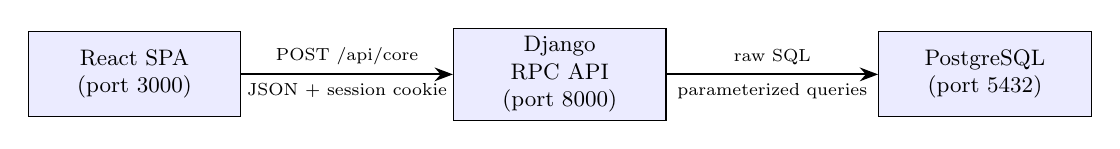
\begin{tikzpicture}[
    box/.style={rectangle, draw, fill=blue!8, minimum width=3cm, minimum height=1.2cm, font=\small, align=center},
    arr/.style={->, thick, >=Stealth},
    scale=0.9, transform shape
]
\node[box] (browser) at (0, 0) {React SPA\\(port 3000)};
\node[box] (django) at (6, 0) {Django\\RPC API\\(port 8000)};
\node[box] (pg) at (12, 0) {PostgreSQL\\(port 5432)};

\draw[arr] (browser) -- node[above, font=\scriptsize] {POST /api/core} node[below, font=\scriptsize] {JSON + session cookie} (django);
\draw[arr] (django) -- node[above, font=\scriptsize] {raw SQL} node[below, font=\scriptsize] {parameterized queries} (pg);
\end{tikzpicture}
\end{center}

\subsection{RPC API Design}

Rather than a RESTful API with multiple endpoints and HTTP verbs, we use a single \textbf{Remote Procedure Call (RPC)} endpoint at \texttt{POST /api/core}. Every request contains a JSON body:

\begin{lstlisting}[language=Python]
{"function": "function_name", "args": [], "kwargs": {}}
\end{lstlisting}

The server dispatches to the named Python function, which executes the corresponding SQL queries and returns the result as JSON. This approach was chosen for simplicity --- the backend is a single \texttt{views.py} file with a function registry, making it easy to add new operations without creating new URL patterns or view classes.

\subsection{Available API Functions}

The system provides \textbf{26 RPC functions} organized into six categories:

\begin{center}
\small
\begin{tabular}{ll}
\toprule
Category & Functions \\
\midrule
Auth (4) & \texttt{register}, \texttt{login}, \texttt{logout}, \texttt{me} \\
Workspaces (8) & \texttt{get\_workspaces}, \texttt{create\_workspace}, \texttt{delete\_workspace} \\
 & \texttt{get\_workspace\_members}, \texttt{invite\_to\_workspace} \\
 & \texttt{respond\_workspace\_invite}, \texttt{update\_workspace\_member}, \texttt{leave\_workspace} \\
Channels (7) & \texttt{get\_channels}, \texttt{create\_channel}, \texttt{delete\_channel} \\
 & \texttt{get\_channel\_members}, \texttt{invite\_to\_channel}, \texttt{respond\_channel\_invite} \\
 & \texttt{join\_channel}, \texttt{leave\_channel}, \texttt{get\_public\_channels} \\
Messages (3) & \texttt{get\_messages}, \texttt{send\_message}, \texttt{search\_messages} \\
Users (1) & \texttt{search\_users} \\
Reports (2) & \texttt{get\_workspace\_admins}, \texttt{get\_pending\_channel\_invites} \\
Admin (1) & \texttt{initialize} \\
\bottomrule
\end{tabular}
\end{center}


\newpage
\section{Implementation Details}
\label{sec:impl}

\subsection{Backend Implementation}

The entire backend is contained in \texttt{DBProject/views.py}. Key implementation choices:

\begin{itemize}
    \item \textbf{Raw SQL only.} Every database operation uses \texttt{connection.cursor()} and parameterized SQL queries. Django's ORM is not used, in compliance with the course requirement. For example, the login function:
\end{itemize}

\begin{lstlisting}[language=Python]
def login(request, email, password):
    with connection.cursor() as c:
        c.execute(
            "SELECT uid, email, username, nickname, pwhash "
            "FROM users WHERE email = %s",
            [email],
        )
        user = _dictfetchone(c)
    if not user or user["pwhash"] != _hash(password):
        return {"error": "invalid credentials"}
    request.session["uid"] = user["uid"]
    return user
\end{lstlisting}

\begin{itemize}
    \item \textbf{Session-based authentication.} Django's built-in session framework stores the user's \texttt{uid} in a server-side session. A session cookie (\texttt{sessionid}) is sent to the browser. Every protected function checks \texttt{request.session.get("uid")} before proceeding.
    \item \textbf{Email-based login.} Users log in with their email address, which is constrained \texttt{UNIQUE NOT NULL} in the \texttt{users} table. This guarantees that login credentials are unambiguous --- no two accounts can share the same email.
    \item \textbf{Password hashing.} Passwords are hashed with SHA-256 (\texttt{hashlib.sha256}) before storage. The hash comparison is performed in Python, not in SQL.
    \item \textbf{Authorization checks.} Operations like \texttt{invite\_to\_workspace} first query the caller's role and verify it is \texttt{'creator'} or \texttt{'admin'} before proceeding.
    \item \textbf{Duplicate prevention.} Workspace and channel invitations use \texttt{INSERT ... ON CONFLICT (wsid, uid) DO NOTHING} to avoid duplicate membership records.
\end{itemize}

\subsection{Frontend Implementation}

The frontend is a React single-page application with the following component hierarchy:

\begin{itemize}
    \item \texttt{App.js} --- top-level routing (login vs.\ chat page); checks session on mount via \texttt{me()}
    \item \texttt{LoginPage.js} / \texttt{RegisterPage.js} --- authentication forms with validation
    \item \texttt{ChatPage.js} --- main layout with state management for workspaces, channels, messages
    \begin{itemize}
        \item \texttt{WorkspaceList.js} --- left sidebar listing workspaces with create button
        \item \texttt{ChannelList.js} --- middle sidebar listing channels with create/browse buttons
        \item \texttt{ChatWindow.js} --- message display with timestamps, per-channel keyword search, and message input with emoji picker
        \item \texttt{Inbox.js} --- dropdown for pending workspace and channel invitations
        \item \texttt{CreateWorkspaceModal.js} --- workspace creation with optional member invites
        \item \texttt{CreateChannelModal.js} --- channel creation (public/private/direct)
        \item \texttt{WorkspaceMembersModal.js} --- member management, role changes, member removal
        \item \texttt{ChannelSettingsModal.js} --- channel member management and deletion
        \item \texttt{DiscoverChannelsModal.js} --- browse and join public channels
    \end{itemize}
\end{itemize}

All API calls go through \texttt{services/api.js}, which wraps the RPC protocol and includes \texttt{credentials: "include"} for session cookie handling across the cross-origin boundary (React on port 3000, Django on port 8000).

\begin{lstlisting}[language=JavaScript]
export const apiCall = async (func, args = [], kwargs = {}) => {
  const res = await fetch(BASE_URL, {
    method: "POST",
    headers: { "Content-Type": "application/json" },
    credentials: "include",
    body: JSON.stringify({ function: func, args, kwargs }),
  });
  const data = await res.json();
  if (!data.ok) throw new Error(data.error || "API error");
  return data.data;
};
\end{lstlisting}

\subsection{Key Features}

\begin{enumerate}
    \item \textbf{User registration and login} --- users create accounts with email, username, nickname, and password, and log in with their email address. Since email is \texttt{UNIQUE NOT NULL}, it unambiguously identifies each account. Sessions persist across page refreshes via the \texttt{me} endpoint.
    \item \textbf{Workspace management} --- create workspaces, invite members (by searching usernames), promote/demote admins, remove members, leave or delete workspaces.
    \item \textbf{Channel types} --- public (discoverable, self-join), private (invite-only), and direct messages (two-person).
    \item \textbf{Messaging} --- send and view messages in real-time within a channel. Messages display chronologically with sender name and timestamp.
    \item \textbf{Invitation inbox} --- pending workspace and channel invitations appear in a dropdown; users can accept or reject each with a single click.
    \item \textbf{Public channel discovery} --- a ``Browse'' button lists public channels in the current workspace that the user has not yet joined. One-click join.
    \item \textbf{Per-channel message search} --- a search icon in the channel header lets users filter messages in the current channel by keyword in real time.
    \item \textbf{Emoji picker} --- an inline emoji picker with categorized Unicode emoji (Smileys, Gestures, Hearts, Objects, Food, Animals, Nature) allows users to insert emoji into messages.
\end{enumerate}


\newpage
\section{Security}
\label{sec:security}

\subsection{SQL Injection Prevention}

All database queries use \textbf{parameterized queries} with \texttt{\%s} placeholders. User-supplied values are never concatenated into SQL strings. Django's database adapter (\texttt{psycopg}) passes parameters separately to PostgreSQL, which treats them as data, not executable SQL.

\begin{lstlisting}[language=Python]
# Safe: parameterized query
c.execute(
    "SELECT uid, email, username, nickname FROM users "
    "WHERE username ILIKE %s OR email ILIKE %s LIMIT 20",
    [f"%{query}%", f"%{query}%"],
)
\end{lstlisting}

The stored procedures defined in \texttt{query.sql} (e.g., \texttt{create\_user}, \texttt{create\_public\_channel}) also use parameterized inputs, providing an additional layer of protection when called directly.

We verified that \textbf{no SQL string concatenation with user input} exists anywhere in the codebase. Every \texttt{c.execute()} call uses \texttt{\%s} placeholders with a parameter list.

\subsection{Cross-Site Scripting (XSS) Prevention}

The frontend uses React, which \textbf{automatically escapes all content rendered in JSX}. When a variable is placed inside curly braces (\texttt{\{msg.content\}}), React converts special characters (\texttt{<}, \texttt{>}, \texttt{\&}, \texttt{"}, \texttt{'}) to their HTML entity equivalents before inserting them into the DOM. This prevents any user-supplied content (message text, usernames, channel names) from being interpreted as HTML or JavaScript.

We do not use \texttt{dangerouslySetInnerHTML} anywhere in the codebase, so there is no bypass of React's built-in XSS protection.

\subsection{Cross-Site Request Forgery (CSRF)}

The RPC endpoint uses \texttt{@csrf\_exempt} because the frontend is a separate React application that communicates via JSON \texttt{POST} requests with session cookies. CSRF protection is mitigated by:
\begin{enumerate}
    \item The endpoint only accepts \texttt{POST} with a \texttt{Content-Type: application/json} header.
    \item Browsers enforce CORS preflight checks for cross-origin JSON requests, preventing third-party sites from forging requests with the correct content type.
    \item Django's \texttt{CORS\_ALLOWED\_ORIGINS} is configured to only allow the frontend's origin (\texttt{http://localhost:3000}).
\end{enumerate}

\subsection{Authentication and Session Security}

\begin{itemize}
    \item \textbf{Server-side sessions.} Django stores session data on the server (in the database by default). Only a session ID cookie is sent to the client.
    \item \textbf{Session cookie security.} The \texttt{sessionid} cookie is HTTP-only and signed by Django's secret key, preventing client-side JavaScript from reading or tampering with it.
    \item \textbf{Authentication guard.} Every protected RPC function checks \texttt{request.session.get("uid")} at the start. If the user is not logged in, an error is returned immediately.
    \item \textbf{Authorization checks.} Role-based operations (e.g., inviting users, promoting admins, deleting workspaces) verify the caller's role in the relevant membership table before proceeding.
\end{itemize}


\newpage
\section{Concurrency and Transaction Safety}
\label{sec:concurrency}

\subsection{Transaction Management}

Multi-step database operations are wrapped in \texttt{transaction.atomic()} to ensure atomicity. If any step fails, the entire transaction is rolled back, preventing partial state changes.

The following operations use explicit transactions:

\begin{itemize}
    \item \texttt{create\_workspace} --- inserts into \texttt{workspaces} and \texttt{workspace\_members} atomically
    \item \texttt{create\_channel} --- checks membership, inserts into \texttt{channels} and \texttt{channel\_members}
    \item \texttt{delete\_channel} --- deletes from \texttt{messages}, \texttt{channel\_members}, and \texttt{channels}
    \item \texttt{delete\_workspace} --- cascading delete across five tables in dependency order
    \item \texttt{invite\_to\_workspace} --- checks role, then inserts invitation
    \item \texttt{update\_workspace\_member} --- checks role, then modifies/removes member
    \item \texttt{initialize} --- drops and recreates all tables with test data
\end{itemize}

Example of a transactional multi-table delete:

\begin{lstlisting}[language=Python]
def delete_workspace(request, wsid):
    uid = request.session.get("uid")
    if not uid:
        return {"error": "not logged in"}
    with transaction.atomic():
        with connection.cursor() as c:
            c.execute("SELECT role FROM workspace_members "
                      "WHERE wsid=%s AND uid=%s", [wsid, uid])
            row = _dictfetchone(c)
            if not row or row["role"] != "creator":
                return {"error": "only the workspace creator can delete it"}
            c.execute("DELETE FROM messages WHERE chid IN "
                      "(SELECT chid FROM channels WHERE wsid=%s)", [wsid])
            c.execute("DELETE FROM channel_members WHERE chid IN "
                      "(SELECT chid FROM channels WHERE wsid=%s)", [wsid])
            c.execute("DELETE FROM channels WHERE wsid=%s", [wsid])
            c.execute("DELETE FROM workspace_members WHERE wsid=%s", [wsid])
            c.execute("DELETE FROM workspaces WHERE wsid=%s", [wsid])
    return {"ok": True}
\end{lstlisting}

\subsection{Isolation Level and Concurrency Guarantees}

PostgreSQL's default isolation level (\texttt{READ COMMITTED}) ensures that concurrent sessions do not see uncommitted changes from other transactions. This prevents issues such as:

\begin{itemize}
    \item A user reading messages from a channel that is being deleted by another user.
    \item Two users simultaneously creating a workspace and both getting the same \texttt{wsid} (prevented by \texttt{SERIAL}).
    \item An invitation being accepted while the workspace is being deleted.
\end{itemize}

Single-statement operations (e.g., \texttt{send\_message}, \texttt{get\_messages}) run in Django's default autocommit mode, which is safe because a single SQL statement is inherently atomic in PostgreSQL.

\subsection{Duplicate Prevention}

The \texttt{INSERT ... ON CONFLICT DO NOTHING} pattern is used for invitations to prevent duplicate membership records when the same user is invited twice:

\begin{lstlisting}[language=Python]
c.execute(
    "INSERT INTO workspace_members (wsid, uid, role, status) "
    "VALUES (%s, %s, 'member', 'pending') "
    "ON CONFLICT (wsid, uid) DO NOTHING",
    [wsid, invitee_uid],
)
\end{lstlisting}

This leverages the composite primary key \texttt{(wsid, uid)} as a natural uniqueness constraint.


\newpage
\section{Deployment}
\label{sec:deploy}

\subsection{Docker Compose Configuration}

The entire backend system runs with a single command: \texttt{docker compose up --build}.

\begin{lstlisting}[language=Python]
# docker-compose.yml (simplified)
services:
  db:
    image: postgres:15
    env_file: .env
    ports: ["5432:5432"]
    volumes:
      - postgres_data:/var/lib/postgresql/data
      - ./sqls/initialize.sql:/docker-entrypoint-initdb.d/01-init.sql
      - ./sqls/insert.sql:/docker-entrypoint-initdb.d/02-insert.sql

  web:
    build: .
    command: ./wait-for-db.sh
    ports: ["8000:8000"]
    depends_on: [db]
    env_file: .env
\end{lstlisting}

\subsection{Startup Sequence}

\begin{enumerate}
    \item PostgreSQL container starts and auto-runs \texttt{initialize.sql} and \texttt{insert.sql} on first boot.
    \item Django container waits for PostgreSQL to be ready (\texttt{wait-for-db.sh} polls port 5432).
    \item Django runs \texttt{migrate} (for session tables) and starts the development server on port 8000.
    \item The user runs \texttt{npm start} in the \texttt{frontend/} directory to start the React development server on port 3000.
\end{enumerate}

\subsection{Environment Variables}

Database credentials are stored in a \texttt{.env} file (not committed to version control):

\begin{lstlisting}
POSTGRES_DB=dbproject
POSTGRES_USER=postgres
POSTGRES_PASSWORD=postgres
POSTGRES_HOST=db
\end{lstlisting}


\newpage
\section{User Guide}
\label{sec:guide}

\subsection{Getting Started}

\begin{enumerate}
    \item \textbf{Start the system:} Run \texttt{docker compose up --build} from the project root.
    \item \textbf{Start the frontend:} In a separate terminal, run \texttt{cd frontend \&\& npm start}.
    \item \textbf{Open the app:} Navigate to \texttt{http://localhost:3000}.
    \item \textbf{Log in or register:} Use a test account (e.g., \texttt{az1234@nyu.edu} / \texttt{alice123}) or create a new account.
\end{enumerate}

\subsection{Main Interface}

The main interface consists of three panels:
\begin{itemize}
    \item \textbf{Left sidebar (purple):} Lists your workspaces. Click to select. The ``+'' button creates a new workspace.
    \item \textbf{Middle sidebar (gray):} Lists channels in the selected workspace. Click to open. Includes buttons for creating channels and browsing public channels.
    \item \textbf{Main area (white/gray):} Displays messages in the selected channel. Type a message and click Send or press Enter. An emoji picker button next to the input allows inserting Unicode emoji.
\end{itemize}

\subsection{Top Bar Actions}

\begin{itemize}
    \item \textbf{Inbox:} Shows pending workspace and channel invitations. Accept or reject each with a single click.
    \item \textbf{Logout:} Ends the session and returns to the login page.
\end{itemize}

\subsection{Workspace Management}

Click ``Members \& settings'' at the bottom of the workspace sidebar to:
\begin{itemize}
    \item View all workspace members and their roles
    \item Invite new members by searching usernames (creator/admin only)
    \item Promote or demote members to/from admin (creator/admin only)
    \item Remove members (creator/admin only)
    \item Leave the workspace (non-creators)
    \item Delete the workspace (creator only --- cascades to all channels and messages)
\end{itemize}

\subsection{Channel Management}

Click ``Channel settings'' at the bottom of the channel sidebar to:
\begin{itemize}
    \item View channel members
    \item Add members from the workspace (channel creator only, for private channels)
    \item Leave the channel
    \item Delete the channel (channel creator only)
\end{itemize}

\subsection{Messaging Features}

\begin{itemize}
    \item \textbf{Send messages:} Type in the input field and press Enter or click Send.
    \item \textbf{Emoji:} Click the emoji button (smiley face) to open a picker with 7 categories (Smileys, Gestures, Hearts, Objects, Food, Animals, Nature). Click any emoji to insert it into the message.
    \item \textbf{Timestamps:} Each message displays the sender's username and the time it was posted.
    \item \textbf{Per-channel search:} Click the magnifying glass icon in the channel header to filter messages in the current channel by keyword.
\end{itemize}


\newpage
\section{Session Logs}
\label{sec:session}

Below are representative session logs demonstrating the core functionality of the system. Each log shows the API calls made and the system's responses.

\subsection{Session 1: Registration and Workspace Setup}

\begin{enumerate}
    \item User opens the registration page and creates an account:
    \begin{itemize}
        \item \texttt{register(email="jd1234@nyu.edu", username="janedoe", nickname="Jane", password="pass123")}
        \item Response: \texttt{\{uid: 9, email: "jd1234@nyu.edu", username: "janedoe"\}}
    \end{itemize}

    \item User creates a new workspace:
    \begin{itemize}
        \item \texttt{create\_workspace(wsname="Study Group", wsdescription="Finals prep")}
        \item Response: \texttt{\{wsid: 4, wsname: "Study Group"\}}
    \end{itemize}

    \item User creates a public channel in the workspace:
    \begin{itemize}
        \item \texttt{create\_channel(wsid=4, chname="algorithms", chtype="public")}
        \item Response: \texttt{\{chid: 12, chname: "algorithms", chtype: "public"\}}
    \end{itemize}

    \item User sends a message:
    \begin{itemize}
        \item \texttt{send\_message(chid=12, content="Who is ready for the algorithms final?")}
        \item Response: \texttt{\{msgid: 121, postat: "2026-04-24T10:30:00"\}}
    \end{itemize}
\end{enumerate}

\subsection{Session 2: Invitations and Collaboration}

\begin{enumerate}
    \item Alice logs in and checks her inbox:
    \begin{itemize}
        \item \texttt{login(email="az1234@nyu.edu", password="alice123")}
        \item \texttt{get\_invitations()} $\Rightarrow$ \texttt{[\{type: "workspace", id: 2, name: "Tandon Robotics Club"\}]}
    \end{itemize}

    \item Alice accepts the workspace invitation:
    \begin{itemize}
        \item \texttt{respond\_workspace\_invite(wsid=2, accept=true)}
        \item Alice can now see channels in the Robotics Club workspace.
    \end{itemize}

    \item Alice browses public channels and joins \#events:
    \begin{itemize}
        \item \texttt{get\_public\_channels(wsid=2)} $\Rightarrow$ \texttt{[\{chid: 5, chname: "events"\}, \{chid: 6, chname: "competitions"\}]}
        \item \texttt{join\_channel(chid=5)} $\Rightarrow$ \texttt{\{ok: true\}}
    \end{itemize}

    \item Alice searches for messages containing ``robotics'':
    \begin{itemize}
        \item \texttt{search\_messages(keyword="robotics")} $\Rightarrow$ Returns results from \#events in WS2 (now accessible after accepting the invite and joining).
    \end{itemize}
\end{enumerate}

\subsection{Session 3: Admin Operations}

\begin{enumerate}
    \item Bob logs in and manages the CS Department workspace:
    \begin{itemize}
        \item \texttt{login(email="bs5678@nyu.edu", password="bob456")}
        \item \texttt{get\_workspace\_members(wsid=1)} $\Rightarrow$ Lists all members with roles.
    \end{itemize}

    \item Bob invites Eve (who has a pending invite) --- no duplicate is created due to \texttt{ON CONFLICT DO NOTHING}:
    \begin{itemize}
        \item \texttt{invite\_to\_workspace(wsid=1, invitee\_uid=5)} $\Rightarrow$ \texttt{\{ok: true\}}
    \end{itemize}

    \item Bob promotes Carol to admin:
    \begin{itemize}
        \item \texttt{update\_workspace\_member(wsid=1, target\_uid=3, role="admin")} $\Rightarrow$ \texttt{\{ok: true\}}
    \end{itemize}
\end{enumerate}

\subsection{Session 4: Direct Messaging}

\begin{enumerate}
    \item Carol logs in and creates a DM with Henry:
    \begin{itemize}
        \item \texttt{login(email="cw9012@nyu.edu", password="carol789")}
        \item \texttt{create\_channel(wsid=3, chtype="direct", invitee\_uid=8)}
        \item Response: \texttt{\{chid: 12, chtype: "direct"\}}
    \end{itemize}

    \item Carol sends a direct message:
    \begin{itemize}
        \item \texttt{send\_message(chid=12, content="Henry, can you push the latest SQL changes?")}
        \item Response: \texttt{\{msgid: 122, postat: "2026-04-24T15:00:00"\}}
    \end{itemize}

    \item Henry logs in and sees the DM:
    \begin{itemize}
        \item \texttt{login(email="hk1234@nyu.edu", password="henry234")}
        \item \texttt{get\_messages(chid=12)} $\Rightarrow$ Returns Carol's message.
    \end{itemize}
\end{enumerate}

\subsection{Session 5: Per-Channel Search}

\begin{enumerate}
    \item Alice opens the DB Project Team workspace and selects \#schema-design:
    \begin{itemize}
        \item \texttt{login(username="alicezhang", password="alice123")}
        \item \texttt{get\_messages(chid=10)} $\Rightarrow$ Returns all messages in \#schema-design.
    \end{itemize}

    \item Alice clicks the search icon in the channel header and types ``BCNF'':
    \begin{itemize}
        \item The message list filters client-side to show only messages containing ``BCNF''.
        \item No additional API call is made --- the filter operates on the already-loaded message list.
    \end{itemize}

    \item Alice clears the search field:
    \begin{itemize}
        \item All messages in \#schema-design are shown again.
    \end{itemize}
\end{enumerate}


\newpage
\section{Design Decisions and Revisions for Project 2}
\label{sec:revisions}

\subsection{Schema Revisions}

The schema from Project~1 was used without structural changes. The \texttt{ON DELETE CASCADE} constraints on foreign keys were already in place, and the \texttt{status} field on membership tables naturally supports the invitation workflow required by the web interface.

\subsection{Design Decisions}

\begin{itemize}
    \item \textbf{RPC over REST.} A single endpoint simplifies both the backend (one URL pattern, one dispatcher) and the frontend (one \texttt{apiCall} helper). Adding a new feature requires only writing a new Python function and decorating it with \texttt{@rpc}.

    \item \textbf{Raw SQL only.} While Django provides a powerful ORM, we exclusively use raw SQL with parameterized queries to satisfy the course requirement and to maintain full control over the generated queries.

    \item \textbf{Session-based authentication over tokens.} Django's built-in session framework provides secure, server-side session management with minimal configuration. The session cookie is HTTP-only and signed, preventing client-side JavaScript from reading the session ID.

    \item \textbf{Application-level cascade deletes.} Although PostgreSQL supports \texttt{ON DELETE CASCADE}, the \texttt{delete\_workspace} and \texttt{delete\_channel} functions explicitly delete dependent rows in order. This gives us full control over the deletion order and allows us to wrap the entire operation in a transaction.

    \item \textbf{Docker Compose for deployment.} The entire system (Django + PostgreSQL) runs with a single \texttt{docker compose up --build} command, making it easy to set up for the demo.

    \item \textbf{Tailwind CSS for styling.} Utility-first CSS framework avoids the overhead of a component library while providing a polished, consistent UI.
\end{itemize}

\subsection{Known Limitations}

\begin{itemize}
    \item No WebSocket support --- the frontend does not receive real-time push updates. Users must refresh or re-select a channel to see new messages.
    \item No message editing or deletion after posting.
    \item No file or image uploads.
    \item Direct channel names are auto-generated as \texttt{DM - username} in the frontend but stored as \texttt{NULL} in the database.
    \item Passwords use SHA-256 hashing rather than a dedicated password-hashing algorithm (e.g., bcrypt). This is acceptable for a course project but not for production use.
\end{itemize}


\newpage
\section{Extra Features}
\label{sec:extra}

The following features go beyond the basic requirements:

\begin{enumerate}
    \item \textbf{Emoji Picker.} The chat input includes an inline emoji picker with 7 categories and over 120 Unicode emoji characters. Users can browse categories (Smileys, Gestures, Hearts, Objects, Food, Animals, Nature) and click to insert. The picker closes automatically when clicking outside.

    \item \textbf{Per-Channel Message Search.} A search icon in the channel header lets users filter the current channel's messages by keyword in real time. The filter operates client-side on the loaded message list with no additional database round-trip.

    \item \textbf{Public Channel Discovery.} A ``Browse Channels'' feature lets users discover and join public channels in their workspaces with a single click, similar to Slack's channel browser.

    \item \textbf{Invitation Inbox.} A unified inbox aggregates pending workspace and channel invitations with accept/reject buttons, providing a streamlined invitation management experience.

    \item \textbf{User Search for Invitations.} When inviting members to a workspace, administrators can search for users by username or email with real-time results, rather than needing to know exact user IDs.

    \item \textbf{Message Timestamps.} Every message displays both the sender's name and the exact timestamp, formatted for readability.

    \item \textbf{Docker Compose Deployment.} One-command setup with \texttt{docker compose up --build} --- no manual database configuration required.
\end{enumerate}


\section{Conclusion}

We have designed and implemented \textit{snickr}, a fully functional web-based collaboration system backed by a PostgreSQL relational database. The system supports user registration, workspace and channel management, role-based access control, invitation workflows, messaging with emoji support, and keyword search --- all through a clean React interface communicating with a Django backend via a single RPC endpoint.

Security measures include parameterized queries against SQL injection, React's automatic XSS escaping, session-based authentication, CORS-restricted API access, and transactional consistency for multi-step operations. The system can be deployed locally via Docker Compose for a live demonstration.

The test dataset includes 8 users across 3 workspaces with 16 channels and over 300 messages, providing rich data for demonstrating all features during the demo.

\end{document}
